\documentclass{IEEEtran}

\usepackage{cite}
\usepackage{amsmath}
\usepackage{amssymb}
\usepackage{url}
\usepackage{graphicx}
\usepackage{booktabs}
\usepackage{microtype}
\usepackage[table]{xcolor}
\usepackage{tikz}
\usetikzlibrary{positioning,arrows.meta,fit,backgrounds}
\usepackage[hidelinks]{hyperref}

\definecolor{phase1blue}{RGB}{52,152,219}
\definecolor{phase2green}{RGB}{46,204,113}
\definecolor{phase3orange}{RGB}{230,126,34}
\definecolor{phase4purple}{RGB}{155,89,182}

\title{Fairness-Aware Routing in Quantum Networks and Clinical Settings\\[0.3em]
{\large\textit{via Multi-Armed, Contextual, and Informative Bandit Methods}}\\[0.3em]
{\large\textit{(Approach Writeup)}}}

\author{%
\begin{minipage}{0.48\textwidth}
\begin{center}
{\bf Piter Z. Garcia}\\
\begin{small}
MS Data Science / Decision-Making \& Algorithmic Fairness\\
Rochester Institute of Technology (RIT)\\
{\it pizg8794@g.rit.edu}
\end{small}
\end{center}
\end{minipage}
\hfill
\begin{minipage}{0.48\textwidth}
\begin{center}
{\bf Dr. Daniel Krutz, Travis Desell}\\
\begin{small}
Department of Software Engineering, Data Science\\
RIT Research Advisors\\
{\it dxkvse@g.rit.edu, tjdvse@g.rit.edu}
\end{small}
\end{center}
\end{minipage}%
}

\begin{document}
\maketitle

%% ─────────────────────────────────────────────────────────────
\section{Approach Overview}
%% ─────────────────────────────────────────────────────────────

Both quantum-network routing and clinical resource allocation are, at their
core, \textit{routing problems}. In quantum networking, entanglement and
qubit resources must be routed across competing flows under probabilistic
link success and scarcity. In clinical settings, diagnostic and treatment
resources must be routed among patients under uncertainty and partial context.
In both cases, \textit{unfair routing is not merely an equity problem; it is
a performance problem}: when a group of flows or patients is systematically
deprioritized, the degradation in success probability, latency, or care
quality is direct and measurable. This shared structure makes the two domains
analytically equivalent and motivates a unified evaluation framework.

The contribution is a reproducible bandit-method framework spanning three
context-richness levels---non-contextual MABs, contextual CMABs, and
informative iCMABs---applied under the same interaction model, fairness-
logging pipeline, and comparison logic in both domains. Two prior works
anchor the testbeds: equitable bioinformatics work provides the clinical
fairness foundation \cite{garcia2025equitable_bioinformatics}, and
threat-aware quantum routing work provides the network environment
\cite{garcia2026threat_aware_quantum_routing}. Quantum networking is a
proven, emerging technology poised to transform communication and resource
allocation; pairing it with clinical fairness---connected through the
structural bridge of routing---positions this work at the intersection of
present human necessity and future breakthrough.

%% ─────────────────────────────────────────────────────────────
\section{Motivating Workflows}
%% ─────────────────────────────────────────────────────────────

\subsection{Clinical Routing Workflow}
The clinical decision-maker routes resources---screens, confirmatory tests,
escalation follow-ups---among patients under incomplete, delayed, or
group-unequal context. Uneven context quality causes the routing policy to
systematically under-resource certain subgroups, producing higher
false-negative rates or inferior downstream care. Clinical fairness is
therefore treated as a time-evolving property of the routing process, not a
static post-hoc audit.

\subsection{Quantum Routing Workflow}
The quantum decision-maker routes entanglement by selecting paths and
allocating scarce entanglement-generation attempts among competing flows
under noisy, stale, or partial context. Unreliable routing context leads to
consistent assignment of degraded paths or resources to certain flow groups,
creating service-equity gaps in success probability, latency, and access.
This makes quantum routing a genuine fairness domain, not merely a
throughput benchmark.

%% ─────────────────────────────────────────────────────────────
\section{Shared Domain Model}
%% ─────────────────────────────────────────────────────────────

The shared domain model (Figure~\ref{fig:domain_model}) organizes the
routing-decision process into four color-coded phases---
\textcolor{phase1blue}{\textbf{Environment}} (blue),
\textcolor{phase2green}{\textbf{Context Observation}} (green),
\textcolor{phase3orange}{\textbf{Routing Decision}} (orange),
\textcolor{phase4purple}{\textbf{Evaluation and Mitigation}} (purple)---
that are structurally identical across both testbeds. Operational semantics
differ: a routing action is a diagnostic decision in the clinical domain and
a path-selection decision in the quantum domain; fairness is measured as
outcome disparity across patient subgroups or network flow groups,
respectively.

%% ─────────────────────────────────────────────────────────────
\section{Design Rationale and Novelty}
%% ─────────────────────────────────────────────────────────────

\subsection{Q1: Why this approach, and why has it not been done before?}
No prior work evaluates fairness-aware sequential routing under a unified
bandit framework spanning clinical and quantum domains. Clinical bandit
research optimizes treatment decisions without modeling routing fairness
across patient subgroups; quantum routing research maximizes throughput
without examining service-equity disparities under partial context. The
critical unaddressed gap is that routing unfairness and routing performance
are inseparable in both domains. Studying them together under a shared
framework---with quantum at the frontier of breakthrough technology and
clinical settings at the frontier of human impact---produces findings that
can improve today's clinical systems and inform the design of fair routing
in tomorrow's quantum-enabled infrastructures.

\subsection{Q2: Why is this approach better than others?}
Single-domain approaches cannot test whether a fairness principle is
structurally general or domain-specific; findings remain unverifiable across
different state spaces, reward structures, and fairness definitions. Post-hoc
fairness audits cannot capture how routing disparities compound over time
under learning. This framework measures fairness at every step under the
same partial-feedback conditions that make routing difficult in practice,
enabling real-time detection, mitigation evaluation, and cross-domain
comparison that no single-domain or post-hoc alternative can provide.

\subsection{Q3: What design and implementation decisions were made, and why?}
\textit{Bandits over full RL:} both domains provide only partial feedback
(the outcome of the chosen route, not counterfactuals), making bandit methods
the correct formulation. \textit{Simulation-first clinical testbed:} a
simulation allows controlled, reproducible injection of missingness, noise,
and group-specific context degradation without sensitive patient data.
\textit{Existing quantum environment extended:} reusing a grounded,
threat-aware quantum routing environment preserves domain realism and avoids
fabricated-testbed credibility risk. \textit{MAB / CMAB / iCMAB spectrum:}
the three levels directly operationalize the core question---whether richer
routing context reduces disparities or amplifies them when context quality
is uneven across groups.

\subsection{Q4: How do these decisions connect to the domain model?}
Each decision maps to a specific phase in Figure~\ref{fig:domain_model}.
The bandit formulation is a \textbf{Phase~3} choice constrained by the
partial-feedback structure of \textbf{Phase~4}. The clinical simulation and
quantum environment extension are \textbf{Phase~1} choices that determine
testbed inputs and conditions. The context spectrum is a \textbf{Phase~2}
choice controlling what routing context is observable and how degraded it
can be. The shared fairness-logging and mitigation loop is a
\textbf{Phase~4} choice ensuring fairness is a per-step first-class output.
The domain model is not a post-hoc diagram; it is the organizational
structure that determined each design choice.

%% ─────────────────────────────────────────────────────────────
\section{Implementation and Evaluation Plan}
%% ─────────────────────────────────────────────────────────────

Both testbeds expose the same policy interface so that MAB, CMAB, and iCMAB
methods are evaluated under a shared logging and analysis pipeline. The
clinical simulation models test ordering, retesting, and escalation decisions
under group-unequal context; the quantum environment models path selection
and entanglement allocation under probabilistic link success and load. The
reward layer tracks accuracy, cost, success rate, and latency; the fairness
layer tracks clinical false-negative and delayed-escalation gaps and quantum
service-equity gaps across flow groups. Experiments run from explicit
configuration files with fixed random seeds and per-step metric logging,
and at least one fairness-aware mitigation mechanism is evaluated within the
same framework to enable direct comparison against baseline policies.

%% ─────────────────────────────────────────────────────────────
\section{Research Contribution}
%% ─────────────────────────────────────────────────────────────

This work makes three contributions. First, it identifies routing as the
structural common ground between clinical and quantum domains and builds the
first fairness-aware sequential decision framework evaluating both under
identical conditions. Second, it provides the first systematic MAB/CMAB/iCMAB
comparison with respect to routing fairness, isolating whether richer context
reduces or amplifies disparities when context quality is uneven. Third, by
connecting a domain of immediate human health impact to a proven breakthrough
technology through their shared routing structure, the findings serve both as
an evaluation of current systems and as a foundation for fair routing in
next-generation quantum-enabled infrastructures.

%% ─── Figure at end — does not count toward two-page limit ───
\begin{figure*}[!b]
\centering
\resizebox{0.97\textwidth}{!}{%
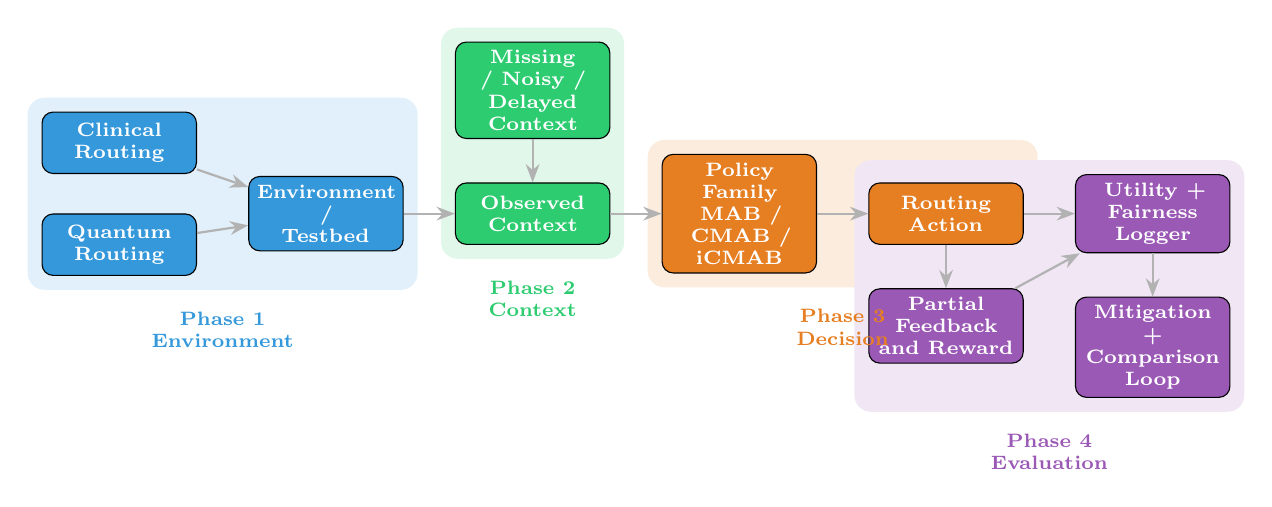
\begin{tikzpicture}[
  font=\scriptsize,
  box/.style={draw, rounded corners=4pt, align=center,
              text width=1.75cm, minimum height=0.78cm,
              inner sep=3pt, text=white, font=\scriptsize\bfseries},
  phase1/.style={box, fill=phase1blue},
  phase2/.style={box, fill=phase2green},
  phase3/.style={box, fill=phase3orange},
  phase4/.style={box, fill=phase4purple},
  arr/.style={-Stealth, thick, gray!60},
  lbl/.style={font=\scriptsize\bfseries, align=center}
]
\node[phase1] (clin)  {Clinical\\Routing};
\node[phase1, below=0.5cm of clin]  (quant) {Quantum\\Routing};
\node[phase1, right=0.65cm of clin, yshift=-0.9cm] (env) {Environment /\\Testbed};
\node[phase2, right=0.65cm of env]  (ctx) {Observed\\Context};
\node[phase2, above=0.55cm of ctx]  (deg) {Missing / Noisy /\\Delayed Context};
\node[phase3, right=0.65cm of ctx]  (pol) {Policy Family\\MAB / CMAB / iCMAB};
\node[phase3, right=0.65cm of pol]  (act) {Routing\\Action};
\node[phase4, below=0.55cm of act]  (fb)  {Partial Feedback\\and Reward};
\node[phase4, right=0.65cm of act]  (log) {Utility + Fairness\\Logger};
\node[phase4, below=0.55cm of log]  (mit) {Mitigation +\\Comparison Loop};

\draw[arr] (clin)--(env); \draw[arr] (quant)--(env);
\draw[arr] (env)--(ctx);  \draw[arr] (deg)--(ctx);
\draw[arr] (ctx)--(pol);  \draw[arr] (pol)--(act);
\draw[arr] (act)--(fb);   \draw[arr] (act)--(log);
\draw[arr] (fb)--(log);   \draw[arr] (log)--(mit);

\begin{pgfonlayer}{background}
  \node[fill=phase1blue!15,   rounded corners=6pt, inner sep=5pt, fit=(clin)(quant)(env)] (bg1) {};
  \node[fill=phase2green!15,  rounded corners=6pt, inner sep=5pt, fit=(ctx)(deg)]         (bg2) {};
  \node[fill=phase3orange!15, rounded corners=6pt, inner sep=5pt, fit=(pol)(act)]         (bg3) {};
  \node[fill=phase4purple!15, rounded corners=6pt, inner sep=5pt, fit=(fb)(log)(mit)]     (bg4) {};
\end{pgfonlayer}

\node[lbl, text=phase1blue,   below=0.15cm of bg1] {\textbf{Phase 1}\\Environment};
\node[lbl, text=phase2green,  below=0.15cm of bg2] {\textbf{Phase 2}\\Context};
\node[lbl, text=phase3orange, below=0.15cm of bg3] {\textbf{Phase 3}\\Decision};
\node[lbl, text=phase4purple, below=0.15cm of bg4] {\textbf{Phase 4}\\Evaluation};
\end{tikzpicture}%
}
\caption{%
  Shared domain model organized into four color-coded phases.
  \textcolor{phase1blue}{\textbf{Phase 1 (blue) --- Environment / Input:}}
    Clinical and quantum routing workflows feed into a shared testbed interface.
  \textcolor{phase2green}{\textbf{Phase 2 (green) --- Context Observation:}}
    Available routing context is observed, subject to missingness, noise, or
    delay---an explicit part of the research question, not an implementation detail.
  \textcolor{phase3orange}{\textbf{Phase 3 (orange) --- Routing Decision:}}
    A policy from the selected method family (MAB, CMAB, or iCMAB) selects a
    routing action under the observed context.
  \textcolor{phase4purple}{\textbf{Phase 4 (purple) --- Evaluation and Mitigation:}}
    Partial feedback is returned; utility and fairness are logged per step;
    baseline and fairness-aware mitigation policies are compared within the same loop.}
\label{fig:domain_model}
\end{figure*}

\begin{thebibliography}{9}\setlength{\itemsep}{0em}
\bibitem{garcia2025equitable_bioinformatics}
Garcia, P. Z. Equitable Bioinformatics: Enhancing Diagnostic
Decision-Making through {RNA} and Biomarker Data. Course paper
(ISTE~780 Phase~4), Rochester Institute of Technology, 2025.
\bibitem{garcia2026threat_aware_quantum_routing}
Garcia, P. Z. Threat-Aware Evaluation of Quantum Entanglement Routing
and Qubit Allocation via Hybrid Contextual Bandits. Unpublished
manuscript, Rochester Institute of Technology, 2026.
\end{thebibliography}

\end{document}
